\documentclass[a4paper,12pt]{jsarticle}


\usepackage[top=30truemm,bottom=30truemm,left=25truemm,right=25truemm]{geometry}
\usepackage{amsmath,amsfonts}
\usepackage{bm}
\usepackage[dvipdfmx]{graphicx}
\usepackage{booktabs}
\usepackage{array}
\usepackage{multirow}
\usepackage{here}
\usepackage{array}
\usepackage{tabu}
\usepackage{wrapfig}
\usepackage{mathcomp}


\begin{document}

\title{光学フィルターと回析格子を用いたプランク定数$h$の測定}
\author{Teduka Yuuki 1522063 
\\
Collaborator:Nakamura Kouta 1522B02, Mizusiri Kenngo 1522089 }
\date{Lab date: 2th and 9th May 2023}
\maketitle

\begin{abstract}
この実験の目的は、プランク定数$h = 6.62607015 \time 10^{-34}$を高い精度で求めることである。\\プランク定数は、照射する光の振動数$\nu$と金属の仕事関数$\phi$を用いて、$h = {eV_t}/{\nu} - {e\phi}/{\nu}$で求められる訳だから、いくつかの光の振動数$\nu$に対して、それぞれの阻止電圧を測定してやれば、$V_t-\nu$グラフの傾きからプランク定数を求めることができる。
実験では、色フィルターと分光計を用いて、白色光を分光し、それぞれの波長の光に対して阻止電圧を測定した。その結果、2つの事が分かった。
一つ目は、$10^{-34}$というオーダーで一致し、実験値はおおよそ文献値に近い値が得られたということである。これは、電流計や
電圧計の誤差や、光電管の温度の影響があった場合でも、今回の実験法ではプランク定数のオーダーを正確に求めることができるということである。
2つ目は、分光計を用いた場合も、厳密に単一の波長だけを照射することは難しく、逆電圧-光電流特性は裾を引くような形になった。
厳密に単一波長だけからなる光を用いた場合は、光を阻止する電圧の増加に伴い、電流は直線的に減少するはずなので、逆電圧-光電流特性グラフは直線上になることが予測されるが、実際の結果で裾を引くのは、実験では単一の波長にするのは難しく、波長が異なる光が混ざってしまったことが原因であると考えられる。
\end{abstract}


\section{Introduction}
光電効果の実験から、プランク定数$h$は、照射する光の振動数$\nu$と金属の仕事関数$\phi$を用いて$h\nu = E + e\phi$で表せることは知っている。光電子の運動エネルギー$E$を直接観測することは難しいので、コレクタに逆電圧をかけて、ポテンシャルエネルギーを観測する。つまり、電子の最大運動エネルギー$E$は、コレクタに到達できなる時の阻止電圧$V_t$を用いて、$E = eV_t$と表せるので、結局$h = {eV_t}/{\nu} - {e\phi}/{\nu}$で求められる。
従って、いくつかの光の振動数$\nu$に対して、それぞれの阻止電圧を測定してやれば、$V_t-\nu$グラフの傾きからプランク定数を求めることができる。

\section{Experimental procedures}
[使用器具]

プランク定数測定装置、白熱燈光源、可動コイル型電流計(100$\mu$Aレンジ)、可動コイル型電圧計(3Vレンジ)、カラーフィルター(赤、橙、緑、青)
\subsection{カラーフィルターによるプランク定数の測定}
プランク定数測定装置と白熱燈光源の間に、赤、橙、青、緑の4種類のフィルターを挟むことで4種類の光に分けて測定した。電圧を操作して電圧計(3Vレンジ)で値を電流計(100$\mu$Aレンジ)でみて記録していき、電流が0になるまで測定した。これを4種類のフィルターで分光を行い、それぞれのデータをプロットした。

\subsection{回析光子によるプランク定数の測定}
実験系を図1に示した。
左上に白色光源が置かれ、その光はスリットを通過した後、一定の角度で反射される。この方法によって、特定の波長の光を光電管に当てることができる。
\begin{figure}[H]
  \centering
  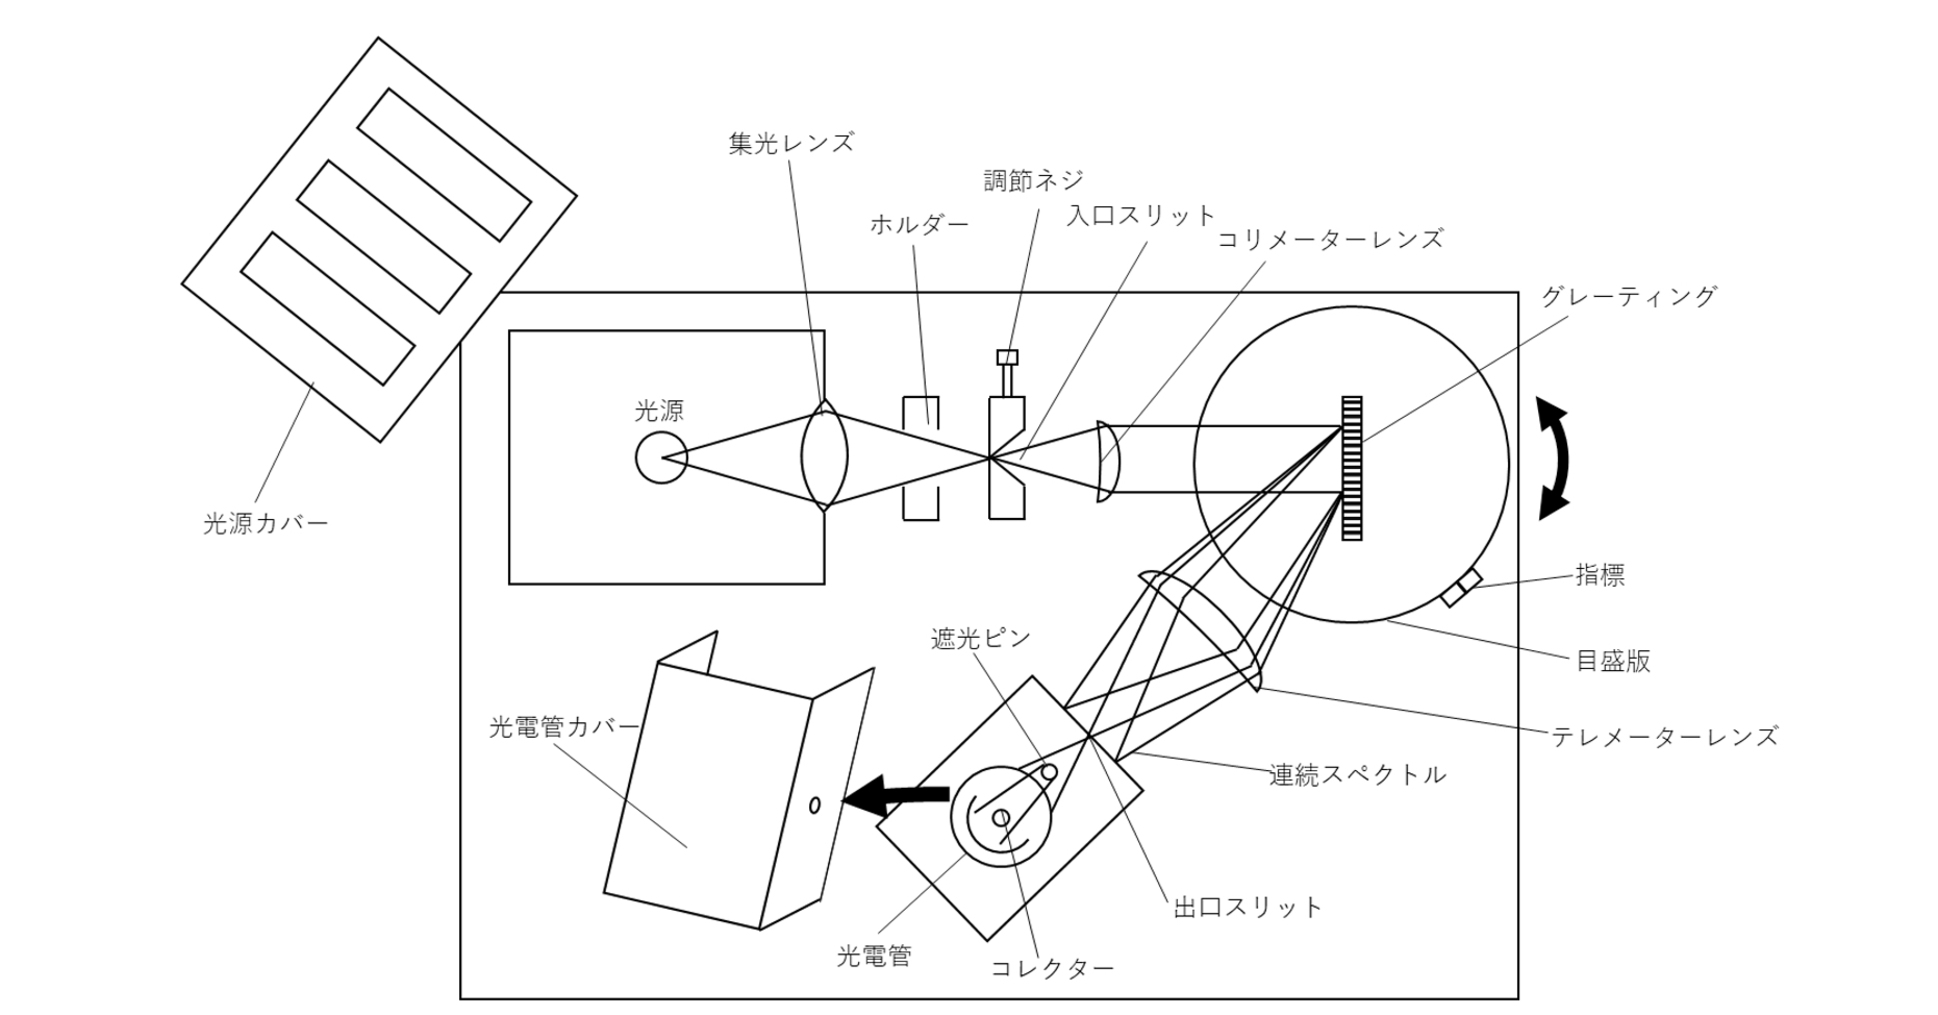
\includegraphics[width=0.9\textwidth]{figs/fig4.pdf}
  \caption{プランク定数の測定の実験装置}
\end{figure}
電圧計と電流計を用いることで、逆電圧をかけた際の光電管に流れる電流を測定した。
電圧値が3.0Vの時に電流計の値が0$\mu$Aになるように調整した。
角度は、0°, -2°, -4°, -6°, -8°の5つの角度で測定した。

\section{Result}
\subsection{カラーフィルターによるプランク定数の測定}
カラーフィルターを通した際の逆電圧‐光電流特性を図2に示した。
波長が短いほど、逆電圧が0Vの際の電流が大きく、電流が0$\mu$Aになるのに必要な逆電圧が大きいことがわかる。
\begin{figure}[H]
\centering
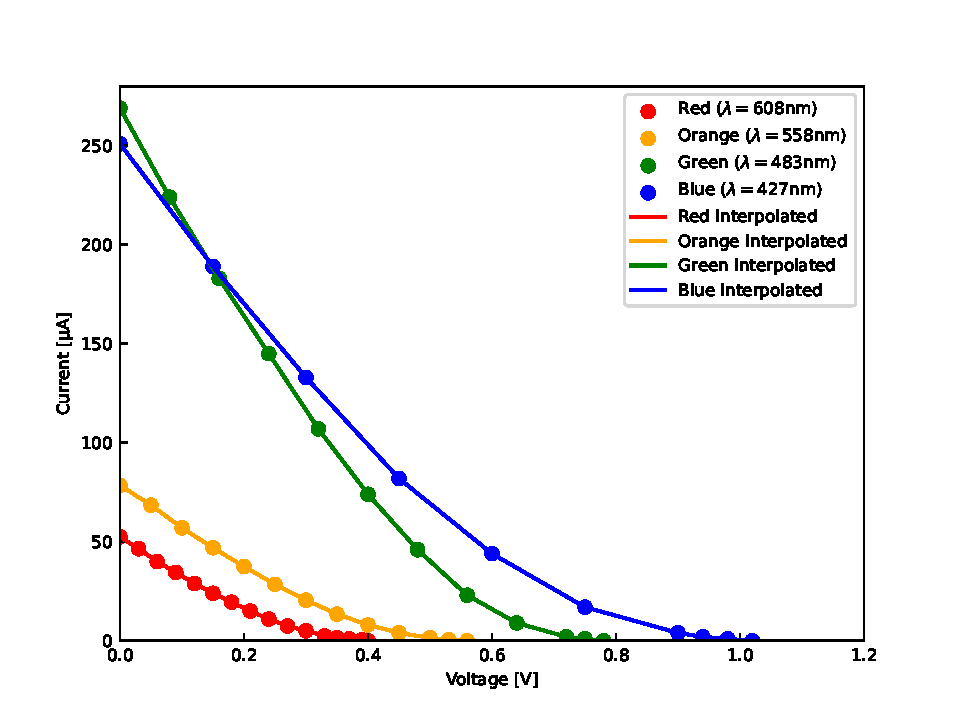
\includegraphics[width=0.7\textwidth]{figs/plot.pdf}
\caption{白色光を4種のカラーフィルターを通した際の電流-電圧特性(縦軸:電流[$\mu$A], 横軸:電圧[V], 赤:赤色フィルター, 青:青色フィルター, 緑:緑色フィルター, 橙:橙色フィルター)}
\end{figure}

\subsection{回析光子によるプランク定数の測定}
分光計を用いて、白色光を分けた際の逆電圧‐光電流特性を図3に示した。
分光計の角度際の波長は凡例の通りである。
実験結果3.1と同様に、波長が短いほど、逆電圧が0Vの際の電流が大きく、電流が0$\mu$Aになるのに必要な逆電圧が大きいことがわかる。
\begin{figure}[H]
  \centering
  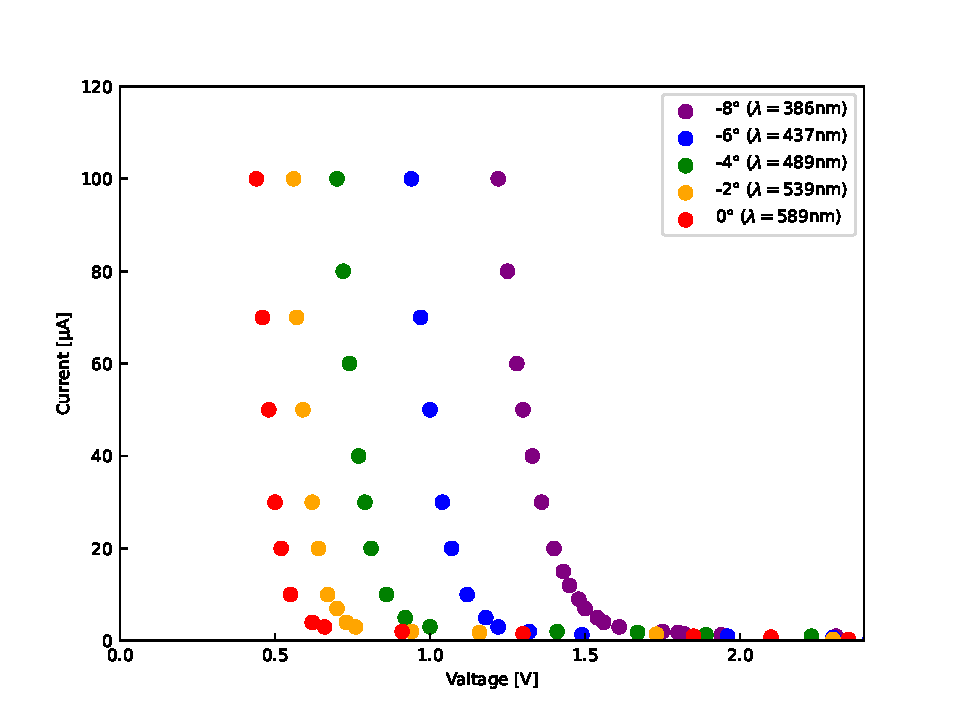
\includegraphics[width=0.7\textwidth]{figs/plot2.pdf}
  \caption{白色光を分光計で光を分けて測定した際の電流-電圧特性(縦軸:電流[$\mu$A], 横軸:電圧[V], 赤:分光計 0°, 橙:分光計 -2°, 緑:分光計 -4°, 青:分光計 -6°, 紫:分光計 -8°)}
  \end{figure}

波長と振動数は反比例の関係にあるので、両者の結果より、波長の減少つまり振動数の増加に伴い、逆電圧の値が増加することがわかる。

\clearpage
\section{Discussion}
\subsection{プランク定数の導出}
得られた電流-電圧特性から、阻止電圧-振動数の関係を求めることで、プランク定数を推定した。
阻止電圧は、電流が0になるときの電圧である。しかし、電流-電圧特性を見ると、直線に近い部分を延長した時の横軸との交点とも見做せるし、電流が流れ始める立ち上がりの部分から考えることもできる。上記の三つの方法でプランク定数を導出し、それぞれの値を比較することで、どの方法が最も正確にプランク定数を導出できるかを考察した。
図4に白色光をカラーフィルターで分光した際の$\nu-V_t$特性を示した。
\begin{figure}[H]
\centering
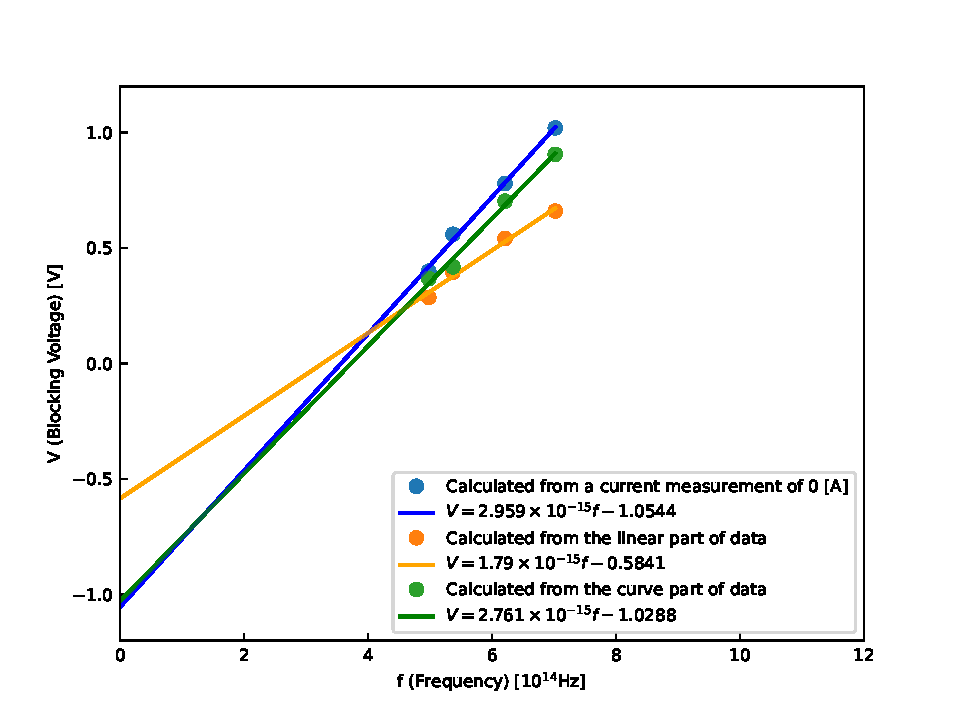
\includegraphics[width=0.7\textwidth]{figs/fitting.pdf}
\caption{白色光を4種のカラーフィルターを通した際の$\nu$-$V_t$特性(縦軸:阻止電圧[V], 横軸:振動数[$\times 10^{14}$Hz], 青:電流の測定値が0の時のデータ, 緑:カーブにした箇所に接線をつけた際のデータ, 橙:データの直線部分を延長した際のデータ)}
\end{figure}
青が電流の測定値が0の時のデータ、橙が直線上に伸ばした時のデータ、緑がカーブに接線をつけた際のデータである。青、緑、橙、赤の4点分のデータから、最小二乗法で傾きを求め、傾きに電気素量$e = 1.602\times 10^{-19}$をかけて、プランク定数を求めた。表1がその結果である。
% Table generated by Excel2LaTeX from sheet '5cm'
\begin{table}[htbp]
  \centering
  \caption{白色光にカラーフィルターを用いた際のプランク定数}
    \begin{tabular}{ll}
    \toprule
    Calculated from a current measurement of 0 [A] & $4.7403\times 10^{-34}$ [J・s] \\
    Calculated from the linear part of data & $2.8676\times 10^{-34}$ [J・s] \\
    Calculated from the curve part of data & $4.4231\times 10^{-34}$ [J・s] \\
    \bottomrule
    \end{tabular}%
  \label{tab:addlabel}%
\end{table}%

プランク定数の文献値は、$6.62607015\times 10^{-34}$ [J・s]である。
一番近い値では、文献値の約1.5倍の誤差があった。しかし、いずれもオーダーは一致しており、$10^{-34}$という非常に小さいスケールで見ると、実験値はおおよそ理想に近い値が得られたと考えられる。

\begin{figure}
  \centering
  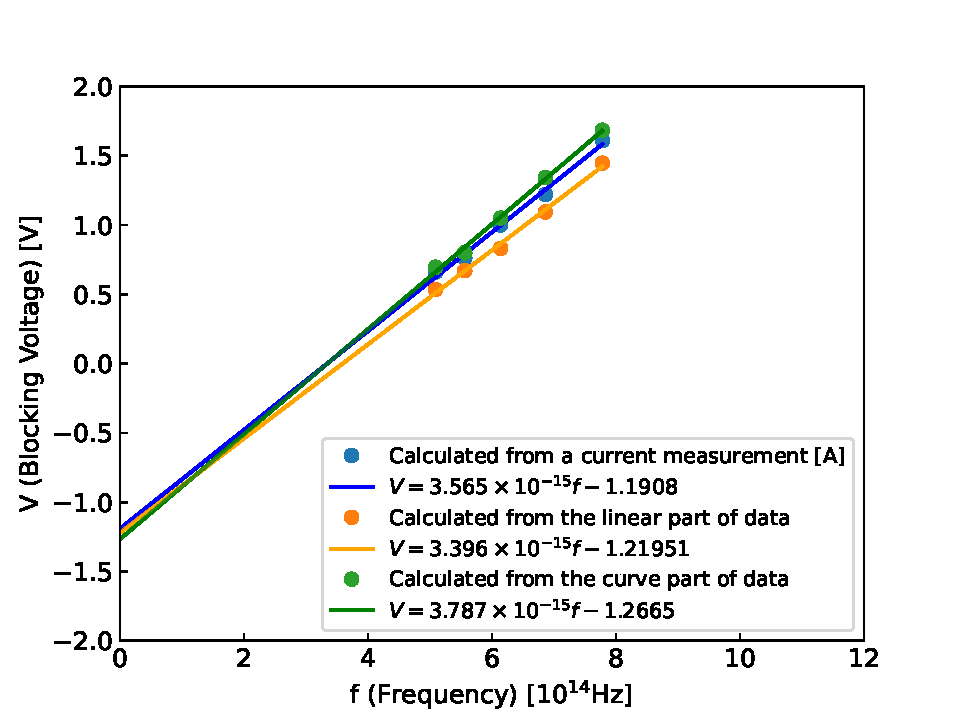
\includegraphics[width=0.7\textwidth]{figs/fitting2.pdf}
  \caption{白色光を分光計で分けた際の$\nu$-$V_t$特性(縦軸:阻止電圧[V], 横軸:振動数[$\times 10^{14}$Hz], 青:測定値から阻止電圧を決めた際のデータ 緑:カーブにした箇所に接線をつけた際のデータ, 橙:データの直線部分を延長した際のデータ)}
\end{figure}
図4は、分光計を用いて白色光を分けた際の$\nu-V_t$特性である。
青が測定から阻止電圧を決定した際のデータである。いずれの波長も、3$\mu$Aの時に光電流が落ち着いていたので、閾値として3$\mu$Aを設定した。
緑がカーブに接線をつけた際のデータ、橙がデータの直線部分を延長した際のデータである。

青、緑、橙、赤の4点分のデータから、最小二乗法で傾きを求め、傾きに電気素量$e = 1.602\times 10^{-19}$をかけて、プランク定数を求めた。表2がその結果である。
\begin{table}[htbp]
  \centering
  \caption{白色光に分光計を用いた際のプランク定数}
    \begin{tabular}{ll}
    \toprule
    Calculated from a current measurement of 0 [A] & $5.71113\times 10^{-34}$ [J・s] \\
    Calculated from the linear part of data & $5.44039\times 10^{-34}$ [J・s] \\
    Calculated from the curve part of data & $6.06677\times 10^{-34}$ [J・s] \\
    \bottomrule
    \end{tabular}%
  \label{tab:addlabel}%
\end{table}%
文献値に一番近い値が$6.06677\times 10^{-34}$で、誤差率は10.9\%であった。カラーフィルターよりも誤差は小さい。

電流電圧特性の曲線的な部分からプランク定数を求める際は、それぞれのデータについて微小変化量、すなわち、$\Delta I / \Delta V$を求め可視化し、非線形な箇所から最小二乗法で傾きを求めた。

\subsection{$\nu$-$V_t$グラフの定数直線と縦軸との交点の原点からの距離の大きさが表すもの}
コレクタの仕事関数を含めて電子のエネルギー図を考える。コレクタはエミッタよりも電子が放出しにくいので、エミッタとコレクタを電気的に接触した場合のエネルギー図は図5のようになる。
コレクタの仕事関数$\phi_C$とエミッタの仕事関数$\phi_E$の差を接触電位という。
\begin{figure}[H]
  \centering
  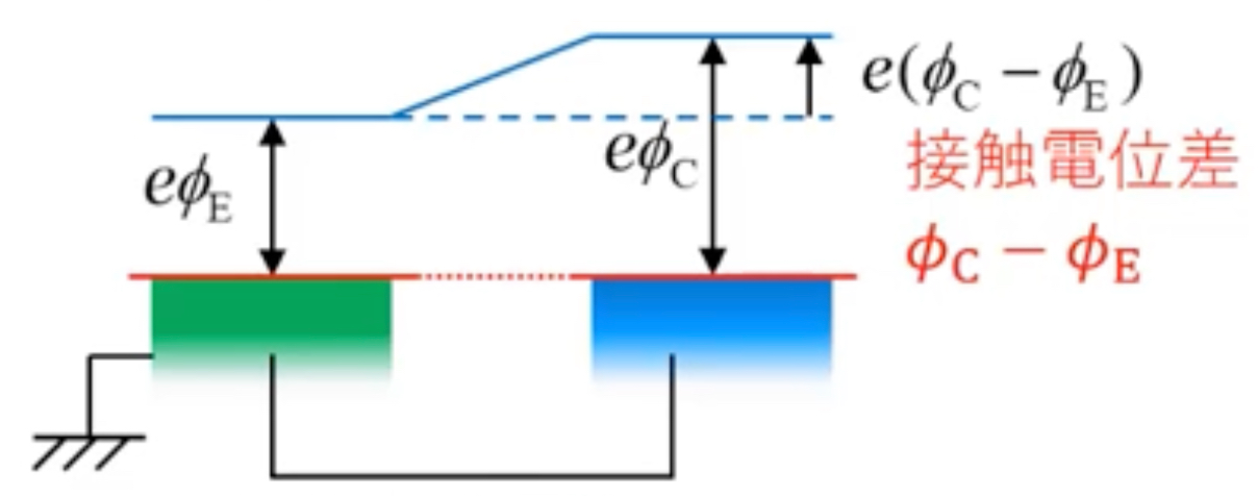
\includegraphics[width=0.35\textwidth]{figs/fig1.pdf}
  \caption{エミッタとコレクタを電気的に接触した場合のエネルギー図(赤線はフェルミ準位)}
\end{figure}

すると、コレクタの仕事関数を含めたエネルギー図は図6のようになる。
\begin{figure}[H]
  \centering
  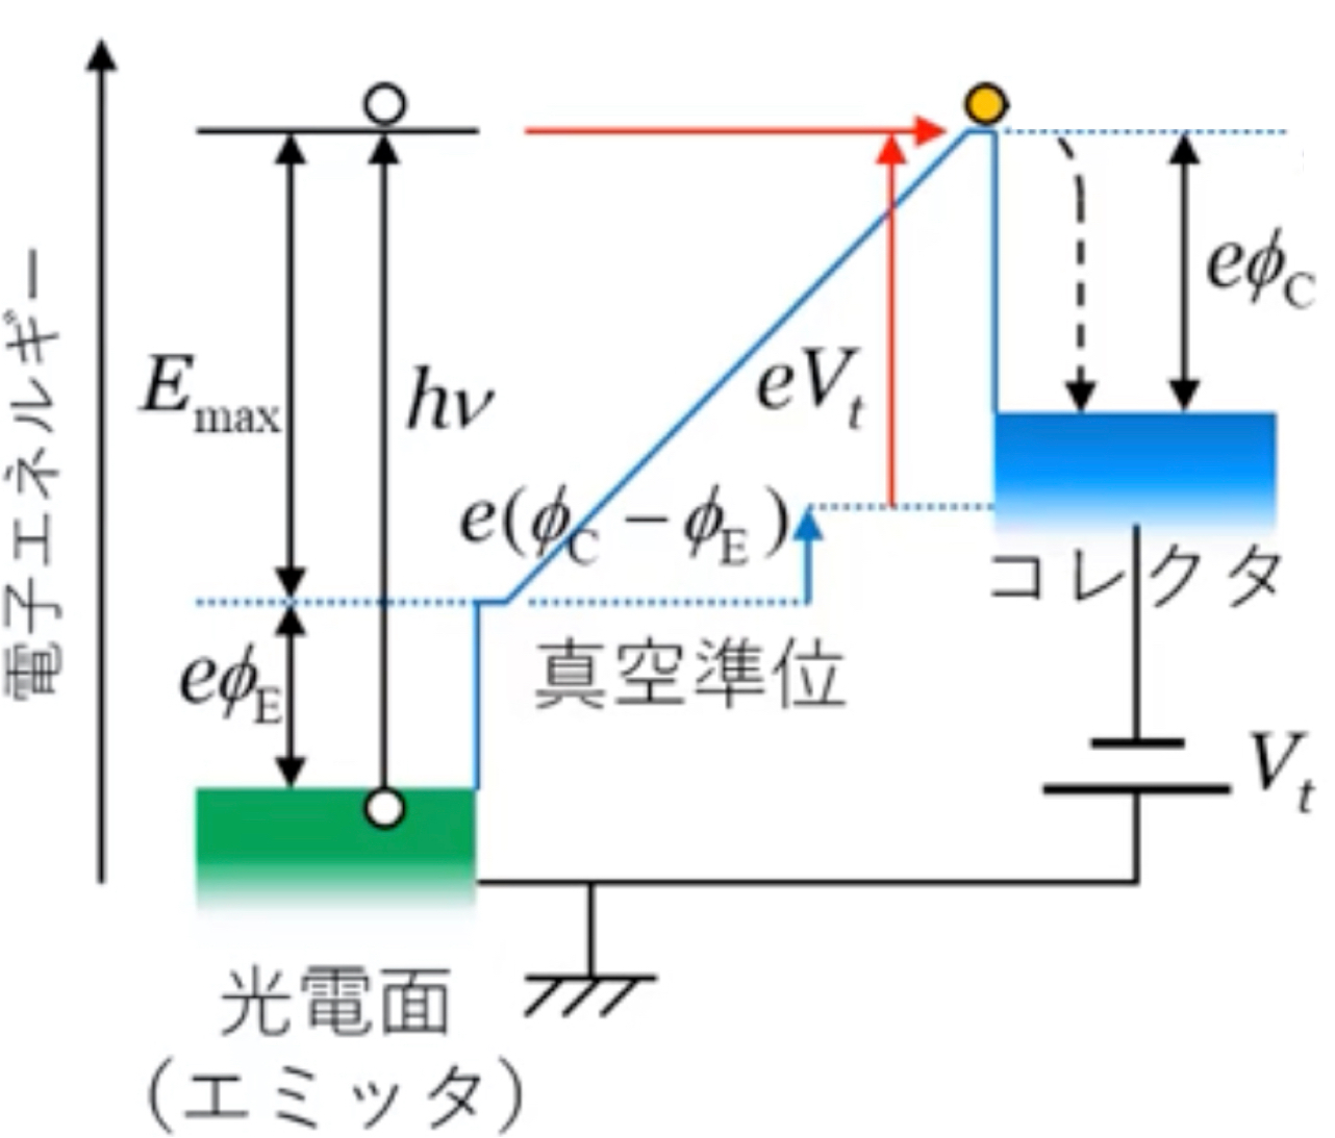
\includegraphics[width=0.35\textwidth]{figs/fig2.pdf}
  \caption{コレクタの仕事関数を含めた場合の電子のエネルギー図}
\end{figure}
光電子はコレクタ付近で運動エネルギーが0なので、図より
\begin{align}
  \begin{split}
  h\nu &= e\phi_E + e(\phi_C - \phi_E) + eV_t \\ 
  &= e\phi_C + eV_t
  \end{split}
\end{align}
となる。すなわち、
\begin{equation}
  V_t = \frac{h\nu}{e} - \phi_C 
\end{equation}
となり、$V_t$-$\nu$グラフの縦軸切片はエミッタの仕事関数ではなく、コレクタの仕事関数を表している事が分かる。
幸い、プランク定数$h$の測定には影響しない。

\subsection{厳密に単一波長だけからなる光を用いた場合の光電流の逆電圧依存性の予測と、実際の実験結果が裾を引く理由}
金属陰局面に一定の振動数の光を照射した場合は、回路に流れる光電流は光の強さにのみ比例する。従って、厳密に単一波長だけからなる光を用いた場合は、光を阻止する電圧の増加に伴い、電流は直線的に減少するはずなので、
逆電圧-光電流特性グラフは直線上になることが予測される。

実際の結果で裾を引くのは、実験では単一の波長にするのは難しく、波長が異なる光が混ざってしまったことが原因であると考えられる。
\subsection{フィルターの特性において、青、緑のフィルターでは短波長側にも透過率が最大値の1/2になる波長があるが、なぜ長波長側ではなく短波長側の透過率が最大値の1/2になる波長を入射光の波長と考えるのか}
光電子の持つ最大のエネルギー$E$は、$E = h\nu = e\phi $で与えられる。
なので、波長が小さい方が光子の持つ最大エネルギーが大きくなることがわかる。波長の最小をとってしまうと、長波長側で光電効果が起こらない。よって短波長側の透過率が最大値の1/2になる波長を入射光の波長と考える。

\section{Conclusion}
光学フィルターと回析格子を用いて白色光を分光し、それぞれの波長の光に対して阻止電圧を測定することで、プランク定数を求めた。
その結果、二つの事が分かった。一つ目は、光学フィルターと回析格子を用いたいずれの場合も、$10^{-34}$ というオーダーで一致し、実験値
はおおよそ文献値に近い値が得られたということである。これは、電流計や電圧計の誤差や、光電管の温度の影響
があった場合でも、今回の実験法ではプランク定数のオーダーを正確に求めることができるということである。二
つ目は、分光計を用いた場合も、厳密に単一の波長だけを照射することは難しく、逆電圧-光電流特性は裾を引くよ
うな形になった。厳密に単一波長だけからなる光を用いた場合は、光を阻止する電圧の増加に伴い、電流は直線的
に減少するはずなので、逆電圧-光電流特性グラフは直線上になることが予測されるが、実際の結果で裾を引くの
は、実験では単一の波長にするのは難しく、波長が異なる光が混ざってしまったことが原因であると考えられる。
\begin{thebibliography}{文献数}
\bibitem{ID} 公益社団法人 日本天文学会:「プランク定数」,天文学辞典
\end{thebibliography}

\end{document}